\begin{figure}[t]
  \centering
  \begin{subfigure}[b]{0.35\textwidth}
    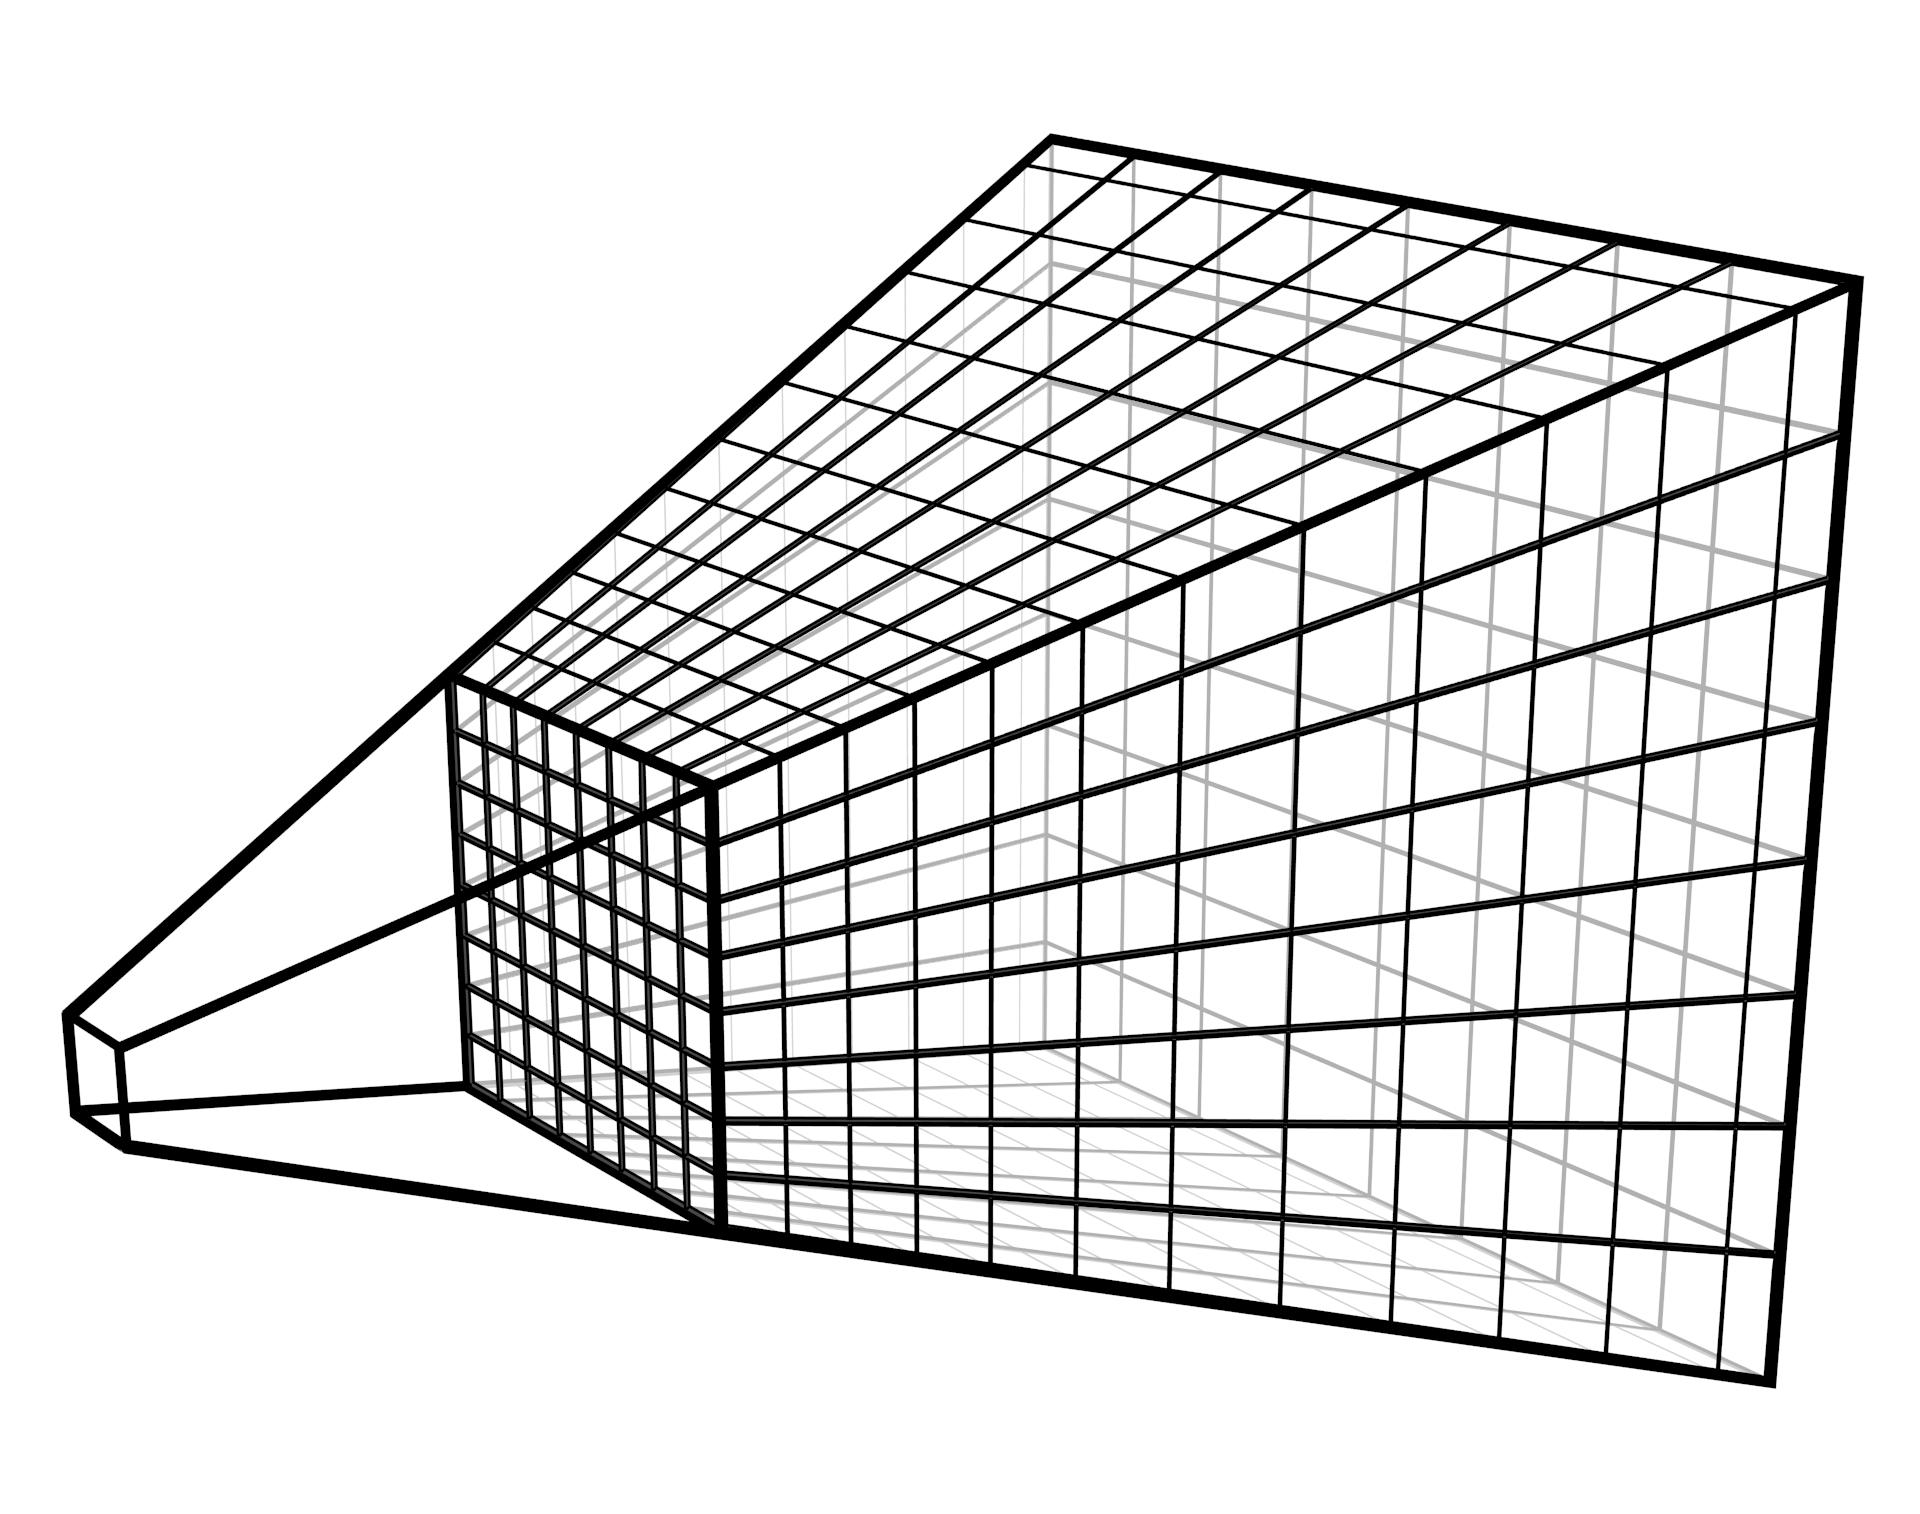
\includegraphics[width=\textwidth]{./img/raw/cs-opdeling-frustum.png}
    \caption{het zichtfrustum}
    \label{fig:cs-opdeling:frustum} %
  \end{subfigure}\quad
  \begin{subfigure}[b]{0.4\textwidth}
    \def\svgwidth{\textwidth}
    \input{./img/raw/cs-sleutel/cs-sleutel2.pdf_tex}
    \caption{Op basis van $h_k$.}
    \label{fig:cs-opdeling:sleutel}
  \end{subfigure}%
  \caption{Opdeling van het zichtfrustum}
  \label{fig:cs-opdeling}
\end{figure}

